\definecolor{c00aeef}{RGB}{0,174,239}
\definecolor{c231f20}{RGB}{35,31,32}
\def \globalscale {1.000000}
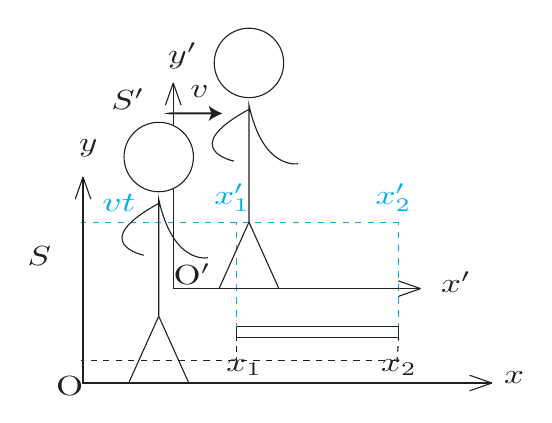
\begin{tikzpicture}[y=1cm, x=1cm, yscale=\globalscale,xscale=\globalscale, every node/.append style={scale=\globalscale}, inner sep=0pt, outer sep=0pt]
  \path[draw=c00aeef,miter limit=10.0] (4.7117, -3.8018) -- (4.7117, -3.7621);
  \path[draw=c00aeef,miter limit=10.0,dash pattern=on 0.0831cm off 0.0831cm] (4.7117, -3.679) -- (4.7117, -2.5569);



  \path[draw=c00aeef,miter limit=10.0] (4.7117, -2.5154) -- (4.7117, -2.4757);



  \path[draw=c00aeef,miter limit=10.0] (2.6535, -3.8018) -- (2.6535, -3.7621);



  \path[draw=c00aeef,miter limit=10.0,dash pattern=on 0.0831cm off 0.0831cm] (2.6535, -3.679) -- (2.6535, -2.5569);



  \path[draw=c00aeef,miter limit=10.0] (2.6535, -2.5154) -- (2.6535, -2.4757);



  \path[draw=c00aeef,miter limit=10.0,dash pattern=on 0.0794cm] (4.7146, -2.4757) -- (0.68, -2.4757);



  \path[draw=c231f20,fill=white,miter limit=10.0] (2.8104, -0.454) circle (0.4408cm);



  \path[draw=c231f20,miter limit=10.0] (2.8104, -2.4757) -- (2.8104, -0.9906).. controls (2.9932, -1.8272) and (3.4348, -1.733) .. (3.4348, -1.733);



  \path[draw=c231f20,miter limit=10.0] (2.8104, -2.4757) -- (2.4305, -3.32);



  \path[draw=c231f20,miter limit=10.0] (2.8104, -2.4757) -- (3.1903, -3.32);



  \path[draw=c231f20,miter limit=10.0] (2.8104, -1.0435).. controls (1.8854, -1.5478) and (2.6204, -1.701) .. (2.6204, -1.701);



  \path[draw=c231f20,miter limit=10.0] (1.8489, -0.708) -- (1.8489, -3.32);



  \node[text=c231f20,cm={ 1.26,-0.0,-0.0,1.0,(0.6535, -1.6489)},anchor=south west] (text9566) at (0.0, 0.0){$y$};



  \node[text=c231f20,cm={ 1.26,-0.0,-0.0,1.0,(1.3962, -1.5579)},anchor=south west] (text2875) at (0.0, 0.0){$S$};



  \path[draw=c231f20,miter limit=10.0] (1.8489, -0.708) -- (1.7497, -0.9893);



  \path[draw=c231f20,miter limit=10.0] (1.8489, -0.708) -- (1.9479, -0.9893);



  \path[draw=c231f20,miter limit=10.0] (4.9887, -3.32) -- (1.8489, -3.32);



  \path[draw=c231f20,miter limit=10.0] (4.9887, -3.32) -- (4.7072, -3.221);



  \path[draw=c231f20,miter limit=10.0] (4.9887, -3.32) -- (4.7072, -3.4192);



  \node[text=c231f20,cm={ 1.26,-0.0,-0.0,1.0,(6.0505, -4.5191)},anchor=south west] (text3754) at (0.0, 0.0){$x$};



  \path[draw=c231f20,fill=white,miter limit=10.0] (1.6645, -1.6489) circle (0.4408cm);



  \path[draw=c231f20,miter limit=10.0] (1.6645, -3.6706) -- (1.6645, -2.1855).. controls (1.8473, -3.0221) and (2.2889, -2.9279) .. (2.2889, -2.9279);



  \path[draw=c231f20,miter limit=10.0] (1.6645, -3.6706) -- (1.2846, -4.5149);



  \path[draw=c231f20,miter limit=10.0] (1.6645, -3.6706) -- (2.0447, -4.5149);



  \path[draw=c231f20,miter limit=10.0] (1.6645, -2.2384).. controls (0.7395, -2.7427) and (1.4745, -2.8959) .. (1.4745, -2.8959);



  \path[draw=c231f20,miter limit=10.0] (0.703, -1.9029) -- (0.703, -4.5149);



  \node[text=c231f20,cm={ 1.29,-0.0,-0.0,1.0,(1.7849, -0.5263)},anchor=south west] (text2515) at (0.0, 0.0){$y^{\prime}$};



  \node[text=c231f20,cm={ 1.26,-0.0,-0.0,1.0,(1.0618, -1.0435)},anchor=south west] (text9280) at (0.0, 0.0){$S^{\prime}$};



  \path[draw=c231f20,miter limit=10.0] (0.703, -1.9029) -- (0.604, -2.1841);



  \path[draw=c231f20,miter limit=10.0] (0.703, -1.9029) -- (0.8022, -2.1841);



  \path[draw=c231f20,miter limit=10.0] (5.8997, -4.5191) -- (0.6842, -4.5191);



  \path[draw=c231f20,miter limit=10.0] (5.8941, -4.5191) -- (5.6129, -4.4199);



  \path[draw=c231f20,miter limit=10.0] (5.8941, -4.5191) -- (5.6129, -4.618);



  \node[text=c231f20,cm={ 1.26,-0.0,-0.0,1.0,(5.2515, -3.3695)},anchor=south west] (text4730) at (0.0, 0.0){$x^\prime$};



  \path[draw=c231f20,miter limit=10.0] (2.6535, -3.8018) -- (4.7117, -3.8018);



  \path[draw=c231f20,miter limit=10.0] (2.6535, -3.8018) -- (2.6535, -3.9415);



  \path[draw=c231f20,miter limit=10.0] (2.6535, -3.9415) -- (4.7117, -3.9415);



  \path[draw=c231f20,miter limit=10.0] (4.7117, -3.8018) -- (4.7117, -3.9415);



  \node[text=c231f20,cm={ 1.26,-0.0,-0.0,1.0,(0.0, -3.0311)},anchor=south west] (text2968) at (0.0, 0.0){$S$};



  \path[draw=c231f20,miter limit=10.0] (2.6535, -3.9415) -- (2.6535, -3.9812);



  \path[draw=c231f20,miter limit=10.0,dash pattern=on 0.0701cm off 0.0701cm] (2.6535, -4.0513) -- (2.6535, -4.1566);



  \path[draw=c231f20,miter limit=10.0] (2.6535, -4.1915) -- (2.6535, -4.2312);



  \path[draw=c231f20,miter limit=10.0] (4.7117, -3.9415) -- (4.7088, -3.9809);



  \path[draw=c231f20,miter limit=10.0,dash pattern=on 0.0693cm off 0.0693cm] (4.704, -4.0502) -- (4.6966, -4.154);



  \path[draw=c231f20,miter limit=10.0] (4.6942, -4.1886) -- (4.6916, -4.228);



  \node[text=c231f20,cm={ 1.26,-0.0,-0.0,1.0,(0.3601, -4.672)},anchor=south west] (text9964) at (0.0, 0.0){O};



  \node[text=c231f20,cm={ 1.26,-0.0,-0.0,1.0,(1.8547, -3.2705)},anchor=south west] (text2136) at (0.0, 0.0){O$^\prime$};



  \node[text=c231f20,cm={ 1.26,-0.0,-0.0,1.0,(2.5247, -4.4257)},anchor=south west] (text19) at (0.0, 0.0){$x_1$};



  \node[text=c00aeef,cm={ 1.26,-0.0,-0.0,1.0,(2.3696, -2.3421)},anchor=south west] (text8886) at (0.0, 0.0){$x_1^\prime$};



  \node[text=c231f20,cm={ 1.26,-0.0,-0.0,1.0,(4.4902, -4.4222)},anchor=south west] (text5227) at (0.0, 0.0){$x_2$};



  \node[text=c00aeef,cm={ 1.26,-0.0,-0.0,1.0,(4.4196, -2.3442)},anchor=south west] (text8645) at (0.0, 0.0){$x_2^\prime$};



  \path[draw=c231f20,miter limit=10.0,dash pattern=on 0.0794cm] (4.6916, -4.228) -- (0.68, -4.228);



  \path[fill=c231f20] (1.7283, -1.0951).. controls (1.7542, -1.0906) and (1.7801, -1.0877) .. (1.806, -1.084).. controls (1.8124, -1.0832) and (1.819, -1.0819) .. (1.8254, -1.0816).. controls (1.8317, -1.0816) and (1.8383, -1.0821) .. (1.8447, -1.0819) -- (2.3498, -1.0819) -- (2.3498, -1.1083) -- (1.8447, -1.1083).. controls (1.8383, -1.1083) and (1.8317, -1.1083) .. (1.8254, -1.1086).. controls (1.819, -1.1083) and (1.8124, -1.107) .. (1.806, -1.1062).. controls (1.7801, -1.1025) and (1.7542, -1.0996) .. (1.7283, -1.0951) -- cycle;



  \path[fill=c231f20] (2.4728, -1.0951).. controls (2.4149, -1.1165) and (2.3432, -1.1533) .. (2.2987, -1.1919) -- (2.3336, -1.0951) -- (2.2987, -0.9983).. controls (2.3432, -1.0372) and (2.4149, -1.0737) .. (2.4728, -1.0951) -- cycle;



  \node[text=c231f20,cm={ 1.26,-0.0,-0.0,1.0,(2.0648, -0.8948)},anchor=south west] (text3953) at (0.0, 0.0){$v$};



  \node[text=c00aeef,cm={ 1.35,-0.0,-0.0,1.0,(0.9485, -2.3421)},anchor=south west] (text8805) at (0.0, 0.0){$vt$};
\end{tikzpicture}